\subsubsection{Block-size-calculation}
Understanding the calculation of Bitcoin block size following the Taproot upgrade is essential.

\paragraph*{block size}

The following illustration depicts the block size calculation:

\begin{figure}[ht] 
    \centering  
    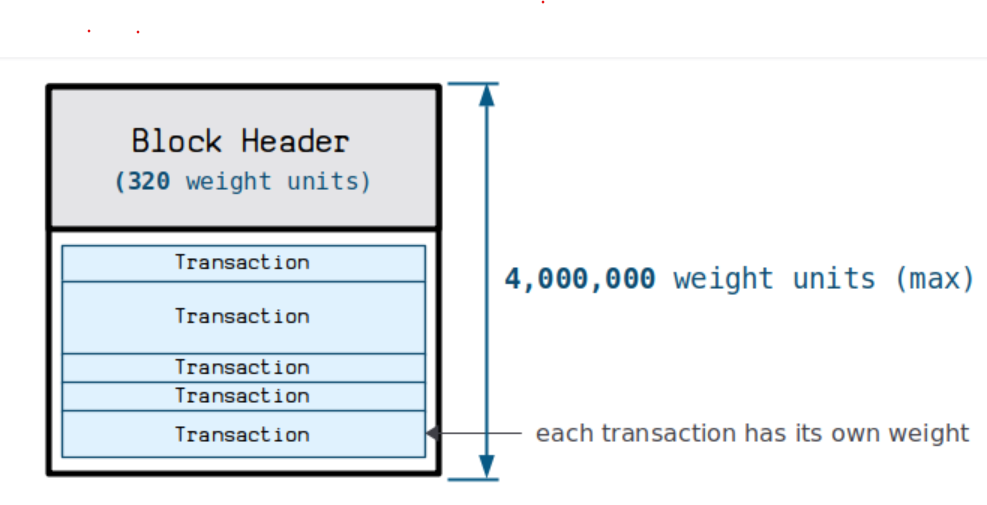
\includegraphics[width=0.85\columnwidth]{images/block-size.png} 
    \caption{Block size}
    \label{fig:block-size}
\end{figure}

\paragraph*{transaction size}

The transaction size calculation is illustrated below:

\begin{figure}[ht] 
    \centering  
    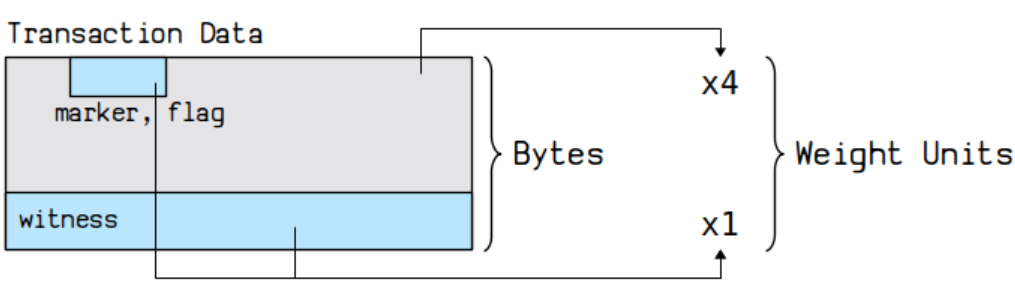
\includegraphics[width=0.85\columnwidth]{images/transaction-size.png} 
    \caption{Transaction size}
    \label{fig:transaction-size}
\end{figure}

For more detailed information, please refer to \cite{website:transaction-size}

\paragraph*{script chunk limitation}

Based on the design of BitVM2 \cite{website:BitVM2}, We aim for each script chunk to be packed into one block as a transaction.
So, the transaction size could not exceed 4,000,000 - 320 = 3,999,680 weight units \cite{website:transaction-size}.

A disputed transaction, characterized by 1 input and 2 outputs, typically has an average non-witness data size of approximately 464 weight units. 
Consequently, the witness size limitation for such transactions is calculated as 3,999,680 - 464 = 3,999,216 weight units.

As outlined in BitVM2 \cite{website:BitVM2}, the disputed transaction needs the signature of Committee, and the signature type is
SIGNHASH\_SINGLE. Let's assume that the number of Committee is 7 and the size of each schnorr signature is 65 bytes (64 bytes for SIGNHASH\_ALL)

So the limitation will be 3,999,216 - 7 * 75 - 8(stack item size) = 3,998,683 weight units.

\begin{figure}[ht] 
    \centering  
    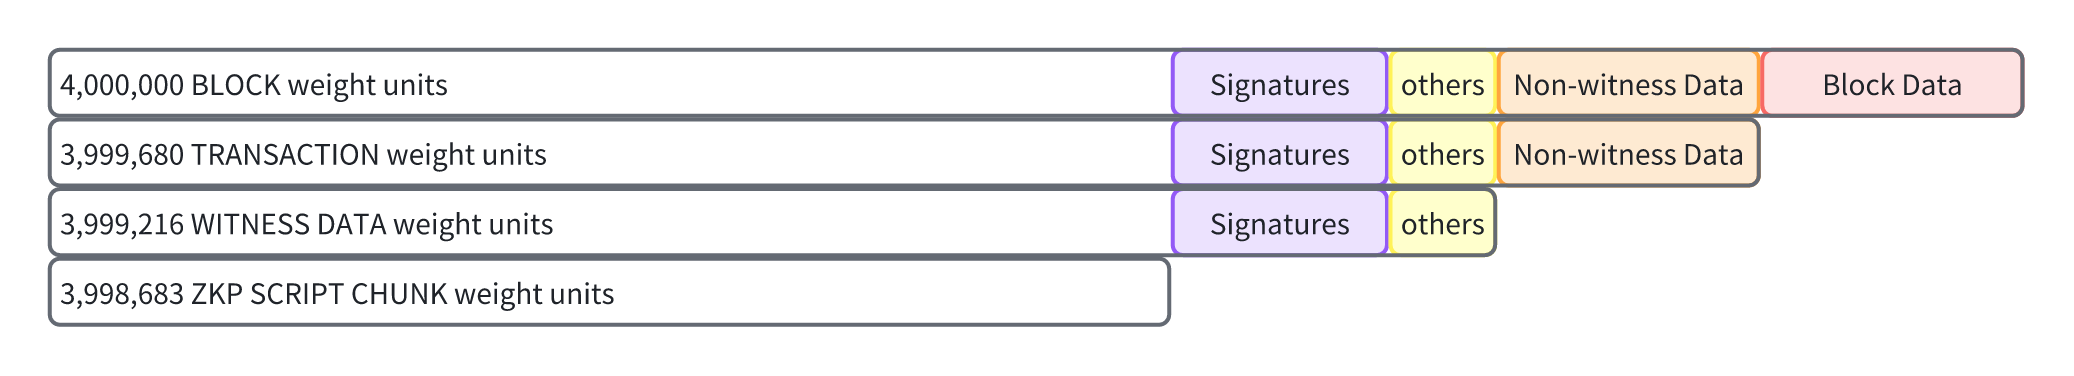
\includegraphics[width=0.85\columnwidth]{images/ZKP-script-chunk-limitation.png} 
    \caption{ZKP script chunk limitation}
    \label{fig:ZKP-script-chunk-limitation}
\end{figure}
